\documentclass[12pt]{article}

\newcommand{\myname}{Tan Yee Jian (A0190190L)}
\newcommand{\mytitle}{CS2309 Homework 3}
\title{\mytitle}
\author{\myname}
\date{\today}

\usepackage[a4paper, total={6in, 9.7in}]{geometry}
\usepackage[utf8]{inputenc}
\usepackage[T1]{fontenc}
\usepackage{textcomp}
\usepackage{amsmath, amssymb, amsthm}
\theoremstyle{plain}
\usepackage[outputdir=tmp]{minted}
\usepackage{graphicx}
% \usepackage{lmodern}
\usepackage{tgpagella}
\usepackage{fancyhdr}
\usepackage{lastpage}
\pagestyle{fancy}
\fancyhf{}
% \rhead{Page \thepage/\pageref{LastPage}}
\rhead{Page \thepage}
\lhead{\myname}
\chead{\mytitle}

\newcommand{\pmat}[1]{ \begin{pmatrix}#1\end{pmatrix} }
\newcommand{\seqn}[1]{(#1)^\infty_{n=1}}
\newcommand{\seqk}[1]{(#1)^\infty_{k=1}}
% (series term): returns a series with counter n=1 to \infty.
\newcommand{\infsrsn}[1]{\sum\limits^\infty_{n=1}#1}
\newcommand{\infsrsk}[1]{\sum\limits^\infty_{k=1}#1}
\newcommand{\R}{\mathbb{R}}
\newcommand{\N}{\mathbb{N}}
\newcommand{\Q}{\mathbb{Q}}
\newcommand{\Z}{\mathbb{Z}}
\newcommand{\C}{\mathbb{C}}
\newcommand{\F}{\mathbb{F}}
\newcommand{\cmm}{C(M_1,M_2)}
\newcommand{\met}[1]{\langle M_{#1},\rho_{#1}\rangle}
\newcommand{\ntoinf}{\limits_{n\to\infty}}
\newcommand{\ktoinf}{\limits_{k\to\infty}}
% \newcommand{\onetoinf}[]{^\infty_{n=1}}
\newcommand{\limn}[1]{\lim\ntoinf #1}
\newcommand{\limk}[1]{\lim\ktoinf #1}

\DeclareMathOperator{\spn}{span}
\DeclareMathOperator{\diam}{diam}

\begin{document}
\maketitle
% \tableofcontents
My favourite presentation in CS2309 (2020/21 Semester 1) is \textbf{Arms Race in
Memory Error Exploit and Defense} by Dr. Liang Zhenkai. His presentation is, in
my opinion, one of the most unique because he has a deeper meaning to convey
behind his presentation, other than the technical details.

\section{What}
\subsection{What was covered}
\label{subsec:description}
The presentation was aimed at students with a simple background in operating
systems and computer organization, which is lower than many of the
machine-learning related talks. He started by explaning what is an activation
record (stack frame) in program execution, and how it can be attacked or
exploited. He then explained that most of the exploits come from the Von Neumann
architecture in computers - instructions as data. Finally, he spends only 6 out
of 45 slides on introducing his research on Data Oriented Programming and how
exploits are constructed in that model, ending with a one-slide case study.

\subsection{What is unique}
\label{subsec:unique}
Most presenters will go on to explain how cool or interesting their projects
are, Dr. Liang has a different aim - he wanted to discuss about his philosophy
towards research, learning and knowledge generation. In the last 9 slides
($20\%$ of the slides), he talked about \emph{Tao}, and how he views learning
and researching on cybersecurity - is about being calm and in deep reflection
with the knowledge that is at hand. He then added a few martial art references
and raises the point of ``counter changes with a constant principle'', asking
the students to ``practice, and most importantly reflect'' with a picture of Jet
Li in the movie \emph{Crouching Tiger, Hidden Dragon (2000)} (Figure
\ref{fig:jet-li}). Finally, he raised the question of (what is) ``the mission of
university education?'' As an ending to his presentation.

\begin{figure}[ht]
  \centering
  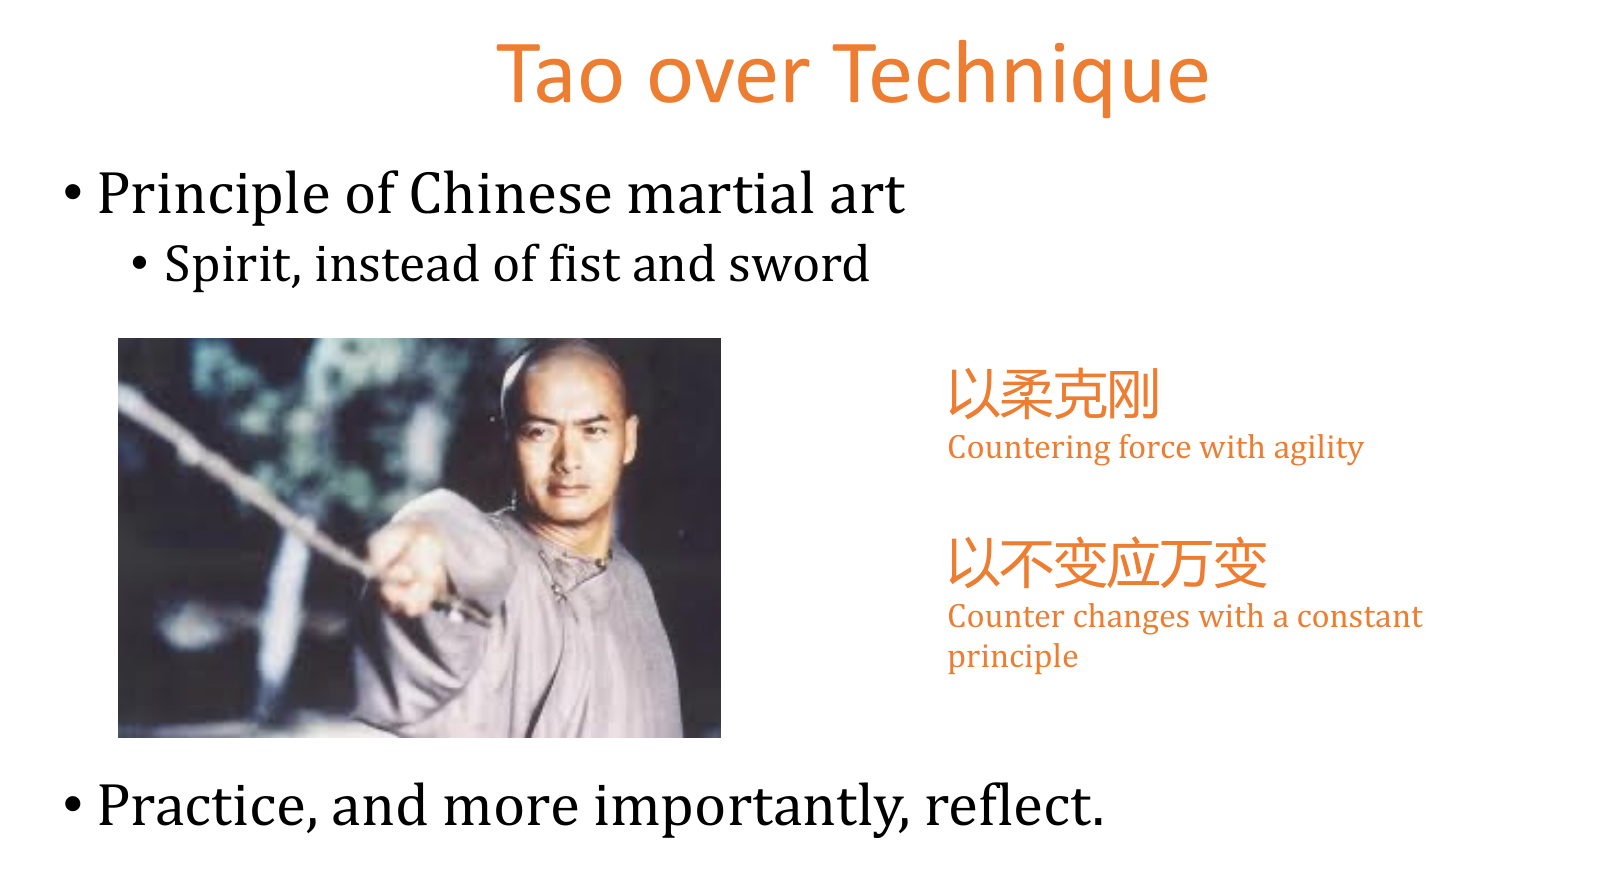
\includegraphics[width=\textwidth]{jet-li.png}
  \caption{\label{fig:jet-li} Tao over Technique. Taken from Prof. Liang
    Zhenkai's slides page 40.}
\end{figure}


\section{Why}
\subsection{Why is this interesting?}
\label{subsec:interesting}
The uniqueness of this presentation lies in this last $20\%$: he prompts us to
reflect about our own learning. Indeed, good research is not only about
hardwork; novel research needs deep reflections about the current situation to
come up with something novel and/or impactful. In a world where an improvement
of $0.1\%$ in testing loss or brute-force parameter tuning are papers of their
own, truly impactful research needs more careful thought.

\begin{figure}[ht]
  \centering
  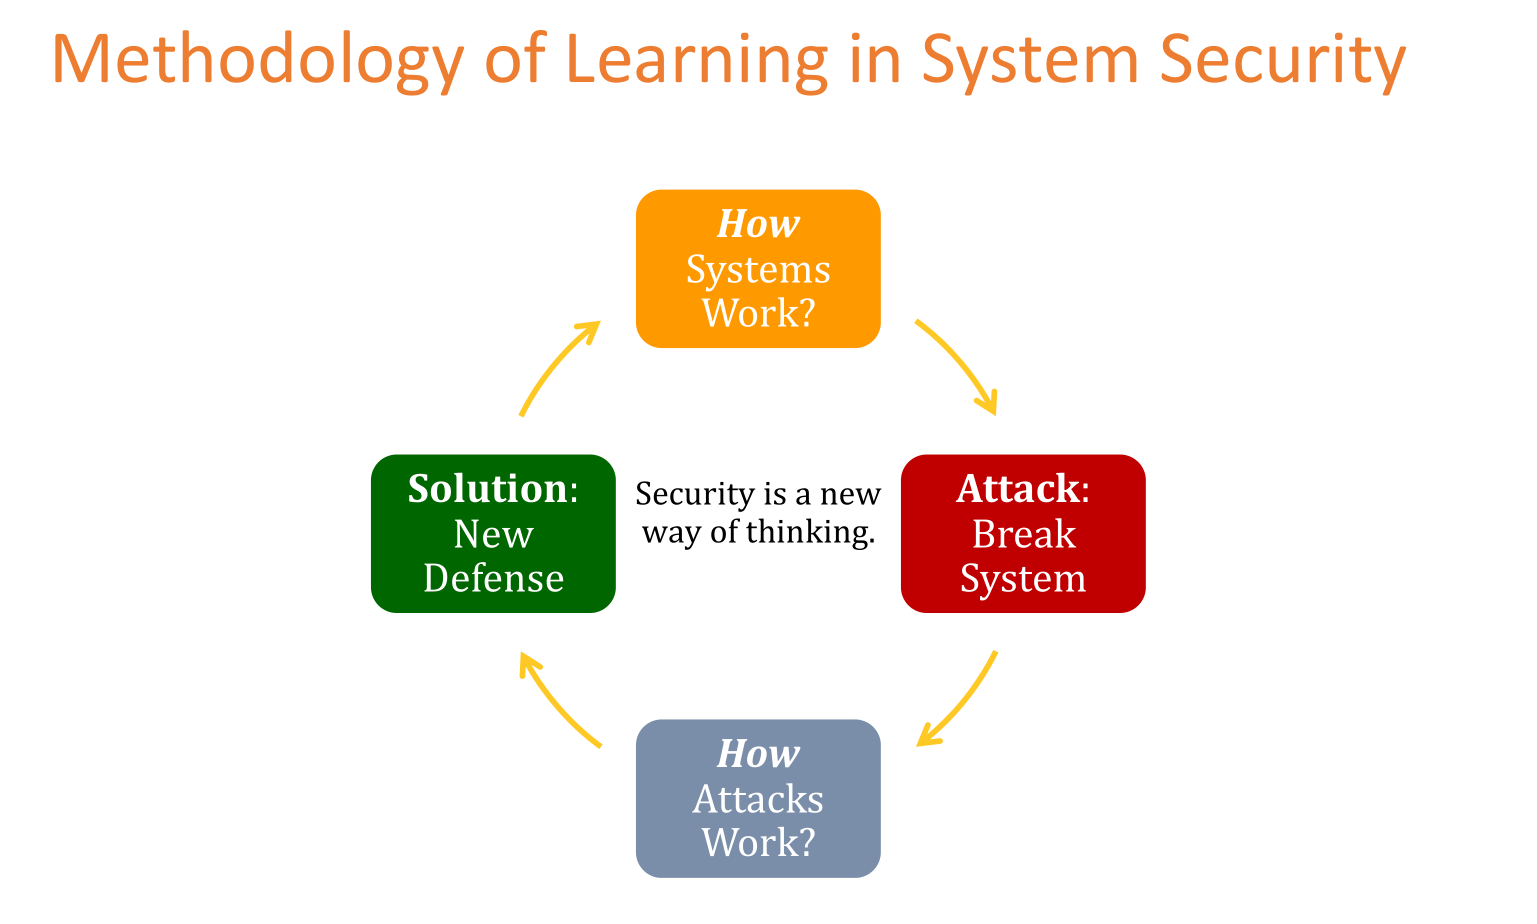
\includegraphics[width=\textwidth]{security.png}
  \caption{\label{fig:security} Security. Taken from Prof. Liang Zhenkai's
    slides page 41.}
\end{figure}

The field of security is best summarized by Figure \ref{fig:security}. More
secure systems need better defense systems, while new defense systems originate
from novel attacks. This require the attacks to be well thought out and be
unique.

Similar to the theoretical research which I am interested in, it is required
that we ask the \textbf{correct} questions to be able to deduce the future
research directions. In this regard, these advice are immensely useful and I
will keep them with me, more than the technical knowledge presented in all the
presentations.

\section{How}
\subsection{How can we learn from this presentation?}
\label{subsec:selection}
In the current situation, it is difficult to cope with the CS2309 assessments
without an ongoing UROPS project. This is because students who still have no
idea what to research on and is purely interested in the area will only have a
semester of self-study before coming up with a research proposal, including a
survey paper and a presentation in between, which is too challenging.
Furthermore, research is about studying the open problems in respective fields,
and by having most of the talk about machine learning is difficult for those who
don't have the required background or not interested in the field.

In contrast, Prof. Liang Zhenkai's talk is very beginner friendly and at most
requires only CS2100 and CS2106 to understand fully. Furthermore, he imparts his
wisdom in research and his own personal thoughts which are very useful to our
growth as both students and potential researchers.

Therefore, in my future presentations, I will take note of not only student's
background knowledge, but also their interests. When the interest is low, some
personal advice and wisdom might be the shining gem in the ashes of nonchalance.


\end{document}
